%!TEX root = ../main.tex

\section{Ziel des Versuchs}
In dem Versuch werden spezifische Eigenschaften von Halbleitern bei verschiedenen Temperaturen untersucht. Die Messungen werden mit Hilfe des Halleffekts durchgeführt und durch dessen Theorie ausgewertet. Bei den Proben Germanium und Galliumarsenid (2DEG) werden von $\SI{-180}{\degree\celsius}$ bis $\SI{150}{\degree\celsius}$ bzw $\SI{0}{\degree\celsius}$ jeweils die Leit- und Hallspannung sowie der dazugehöre Strom aufgezeichnet. Die bestehenden Theorien sollen somit bestätigt werden.

\section{Leitfähigkeit von Halbleitern}

Wir betrachten Halbleiter als kristalline Festkörper mit räumlich periodischer ANordnung der Atome. Diese werden durch eine Gitterkonstate $a$ beschrieben. Man kann dieses Gitter auch im reziproken Raum beschreiben durch den Wellenvektor $\Vec{K}$ mit der Dimension einer inversen Länge. Hierin wird die sogennante Brillouin-Zone definiert, mit allen Punkten im reziproken Raum, die zum Ursprung an nähesten liegen. Dessen Grenzen sind sind bei einem kubischen Gitter gegeben durch:
\begin{align}
    -\frac{a}{\pi} \leq k_i \leq \frac{a}{\pi}
\end{align}
\\
Zur Beschreibung von Elektronen in Festkörpern kann das sogenannte \textbf{Bändermodell} herrangezogen werden. Hierbei kann zwischen verschiedenen Methoden zur Berechnung unterschieden werden, wir beschränken uns nur aus das \textbf{fast freie Elektronenmodell}. Dieses betrachtet die Atomrümpfe im Gitter als ein schwaches periodisches Coulomb-Potential. Ohne Störung kann man die Schrödingergleichung mit einer ebenen Welle analytisch Lösen zu:
\begin{align}
    E(\Vec{k}) = \frac{\hbar^2\Vec{k}^2}{2m_e}.
\end{align}
Betrachtet man nun das Problem mit Potential muss man zur entarteten Störungstheorie greifen. Für konstruktive Interferenz der Streung muss ferner die Lau-Bedingung erfüllt sein. An den Rändern der Brillouin-Zonen gibt es je zwei Lösungen und es entstehen \textbf{Bandlücken}. In Abbildung $\autoref{fig:mod}$ erkennt man die resultierende Energiedispersion mit der Laue-Bedingung $ \Vec{k} = \Vec{k}' + \Vec{G}$ und reziprokem Gittervektor $\Vec{G} = \frac{2 \pi}{a} \cdot n$.
\begin{figure}
    \centering
    \caption{Erweitertes (a) und reduziertes (b) Zonenshema bei fast freien Elektronen. Im Vergleich dazu ein Modell mit einzelnen Atomorbitalen (d) und überlappenden Orbitalen.}
    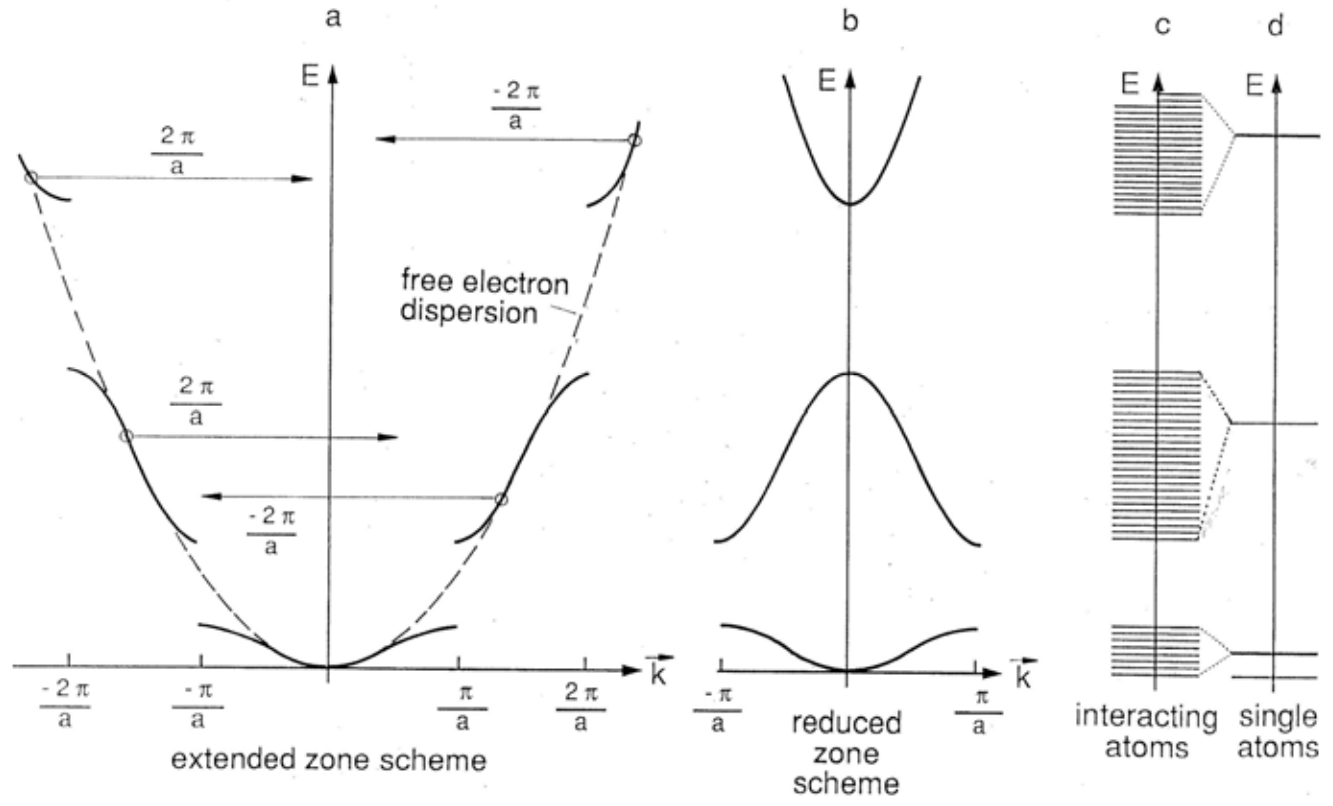
\includegraphics[width=0.8\textwidth]{./fig/band_mod.png}
    \label{fig:mod}
\end{figure}
Um die Bänder nun mit Elektronen zu befüllen muss die \textbf{Fermi-Dirac Statistik} verwendet werden. Wir betrachten die Energieniveaus für $ T = 0$. Der höchste besetzte Zustand hat per Definition die Fermi-Energie. Das letzte vollständig besetzte Band nennt man Valenzband und das darüberligende Band ist das Leitungsband. Es gilt vereinfacht, dass ein vollständig gefülltes Band nicht zur Leitfähigkeit beitragen kann, somit lassen sich drei Fälle unterscheiden:
\begin{itemize}
    \item \textbf{Metalle}: Liegt die Fermienergie innerhalb eines Bandes so handelt es sich um ein Metall. Die jeweiligen Bänder sind somit nur teilweise besetzt und tragen zur Leitfähigkeit bei. \\
    \item \textbf{Isolatoren}: Wenn die Fermienergie dagegen zwischen zwei Bändern liegt kann es sich um einen Isolator oder Halbleiter handeln. Alle Bänder sind entweder vollständig besetzt oder leer. Bei Isolatoren ist die Bandlücke zwischen Valenz- und Leitungsband größer als $E_g > \SI{4}{eV}$. \\
    \item \textbf{Halbleiter}: Betrachtet man nun den Fall für Isolatoren mit einer geringeren Bandlücke als $E_G \leq \SI{4}{eV} $ so handelt es sich um einen Halbleiter. Eine äußere Anregung der Elektronen ist möglich um eine Leitfähigkeit herrzustellen.\\
\end{itemize}

Für die Landungsträger des Halbleiters, also Elektronen und Löcher mit parabolischer Dispersion folgt eine Zustandsdichte der Form $ D(E) \propto \sqrt{E}$ in drei Dimensionen.
\\
\\
Betrachtet man nun den Fall endlicher Temperaturen in Halbleitern so können Leitungsbänder gefüllt und Valenzbänder geleer werden. Dabei ist es sinnvoll das Konzept der Löcher einzuführen, diese entsprechen den Fehlenden Elektronen im Valenzband und tragen via Löcherleitung zum Stromtransport bei. Analog dazu tragen die Elektronen oberhalb der Fermienergie im Leitungsband via Elektronenleitung zum Stromtransport bei. Innerhalb des Kristalls haben diese Quasiteilchen eine effektive Masse der Form:
\begin{equation}
    m^*_{ij}(\Vec{k)} = \frac{\hbar^2}{\frac{d^2E(\Vec{k)}}{dk_i dk_j}}
\end{equation}
hierraus erkennt man die Abhängigkeit der effektiven Masse von der Bandkrümmung. Des weiteren haben Löcher eine negative effektive Masse. \\
\\
Um nun Landungsträger zu erzeugen, bzw. anzuregen gibt es verschiedene Möglichkeiten:

\begin{itemize}
    \item \textbf{Thermische Anregung aus dem Valenzband}: Bei endlichen Temperaturen wird ein geringer Teil der Elektronen aus dem Valenzband in das Leitungsband angehoben. Es entsteht sowohl Löcher- als auch Elektronenleitung. Grundsätzlich kann man für die Elektronen- und Löcherkonzentration n und p folgende Aussage treffen:
    \begin{align}
        n = p = n_i(T).
    \end{align}
    Dieser Effekt dominiert im intrinsischen Bereich und $n_i(T)$ wird daher auch intrinsische Landungsträgerkonzentration genannt. \\
    \item \textbf{Dotierung}: Durch negative oder positive Dotierung eines Halbleiters kann man ein Subenergieniveau erzeugen. Diese liegen näher am jeweiligen Band und können daher viel stärker thermisch Angeregt werden. Es zeichnet sich ein extrinsischer Bereich ab, bei dem dieser Effekt dominiert. Im thermodynamischen Gleichgewicht gilt:
    \begin{align}
        n \cdot p = n_i^2(T).
        \label{eq:dot}
    \end{align}
    Man kann daher einen Halbleiter nur entweder mit Donatoren oder Akzeptoren dotieren. \\
    \item \textbf{Optische Anregung}: Durch optische Anregung können bei Photonenenergien Oberhalb der Bandlücke die Elektronen aus dem Valenzband ins Leitungsband gehoben werden. Ein analogen Effekt hat auch die Ladungsträgerinjektion in einem p-n Übergang. Es herrscht kein thermodynamisches Gleichgewicht mehr.
\end{itemize}

\begin{figure}
    \centering
    \caption{Energieniveaus in n und p dotierten Halbleitern}
    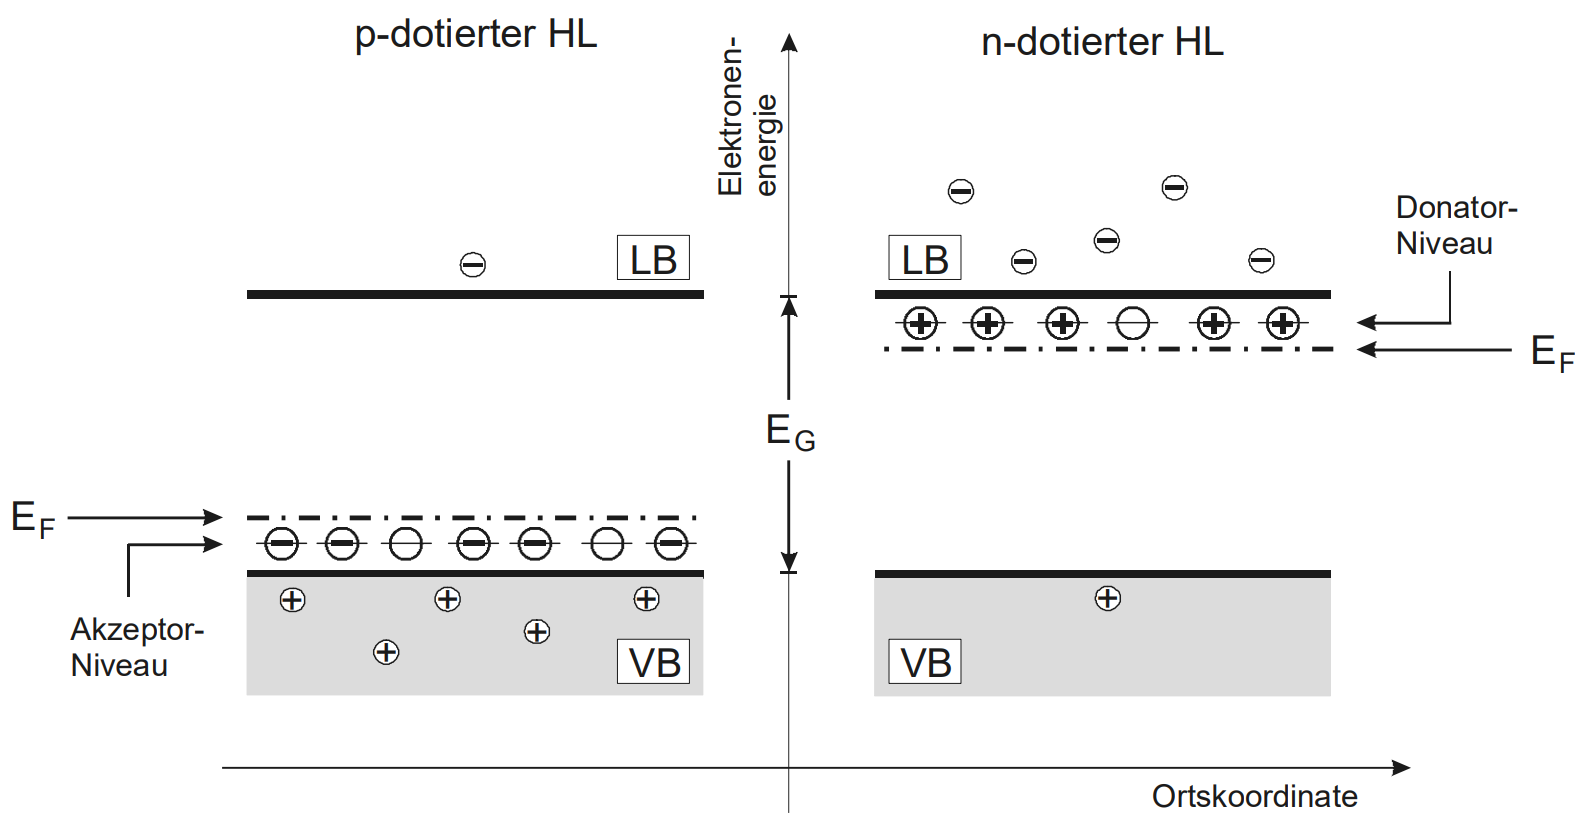
\includegraphics[width=1.0\textwidth]{./fig/hl_dot.png}
    \label{fig:hle}
\end{figure}
Die Elektronen- und Löcherkonzentration ist gegeben durch:
\begin{align}
    n &= \int^{\infty}_{E_L} D(E) f_{FD}\left (\frac{E-E_F}{k_b T} \right) dE \\
    p &= \int_{-\infty}^{E_V} D(E) \left[1-f_{FD}\left (\frac{E-E_F}{k_b T} \right)\right] dE.
\end{align}
Es entsprechen $D(E)$ der Zustandsdichte, $E_L / E_V$ der Leitungsband- Valenzbandkantenenergie und $f_{FD}$ der Fermi-Dirac Verteilung. Letztere beschreibt die Besetzungswahrscheinlichkeit und kann für $E_V \ll E_F \ll E_L$ (wobei sich $\ll$ auf die thermische Energie $k_B T$ bezieht) durch die klassische Boltzmann-Verteilung $f_B$ ersetzt werden. Diese Näherung beschreibt den Fall des \textbf{nichtentarteten Halbleiters}, hierbei Verhalten sich Elektronen und Löcher wie ein klassisches Gas und nicht mehr wie Quasiteilchen. \\
\\
Löst man die Integrale, kann man die Intrinsische Ladungsträgerkonzentration aus Gleichung $\autoref{eq:dot}$ bestimmen zu:
\begin{align}
    n_i(T) = Const \cdot T^{3/2} \cdot exp \left (-\frac{E_G}{2k_bT} \right ).
\end{align}
Der gesamte Verlauf der Landungsträgerkonzentration ist dagegen etwas komplizierter und kann am Beispielt von n dotiertem Germanium gezeigt werden (siehe Abbildung $\autoref{fig:gerdot}$).

\begin{figure}
    \centering
    \caption{Ladungsträgerkonzentration von Germanium}
    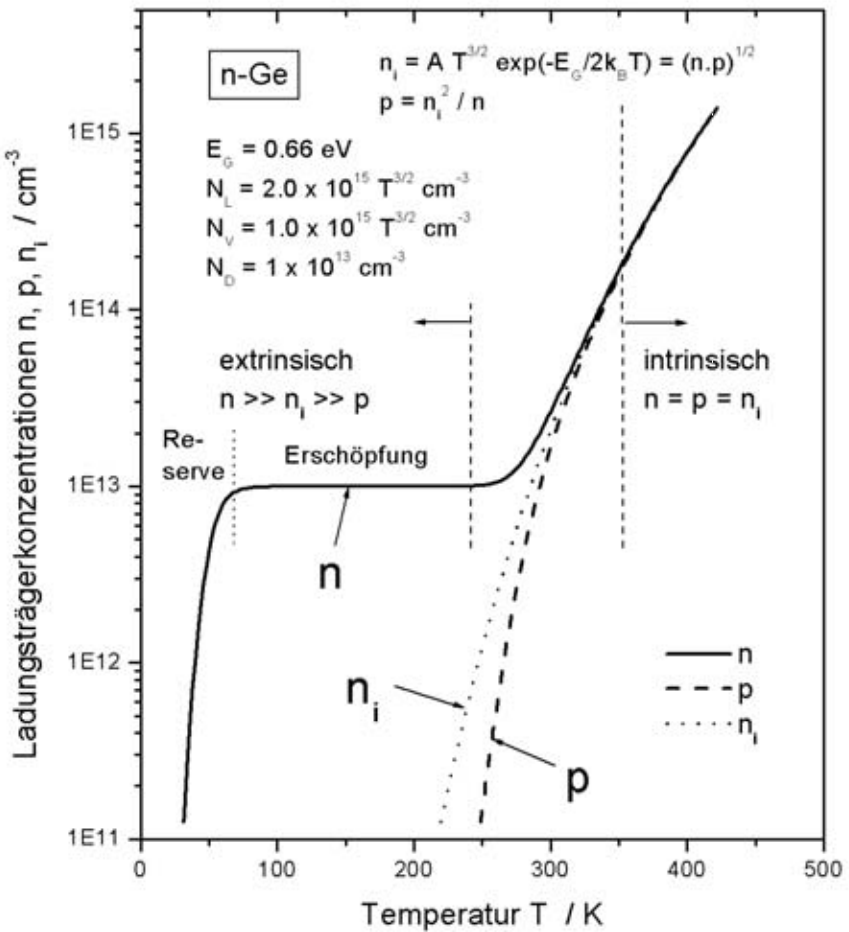
\includegraphics[width=0.6\textwidth]{./fig/ladung_ger.png}
    \label{fig:gerdot}
\end{figure}
Im Reservebereich werden die Donatorelektronen zunehmen thermisch ins LB angeregt, im Erschöpfungsbereich sind bereits alle Donatorelektronen angeregt, diese Bereiche entsprechen dem extrinsischen Verhalten. Steigt die Temperatur noch weiter an begibt sich der Halbleiter in den intrinsischen Bereich.
\\
\\
Die Leitfähigkeit eines Halbleiters kann mittels der Drude-Theorie bestimmt werden. Diese folgt aus dem Ohmschen Gesetzt zu:
\begin{align}
    \sigma = en\mu = e( n\mu_n + h \mu_h)
\end{align}
wobei $\mu$ der Beweglichkeit entspricht, $n$ der Konzentration und $e$ die Elementarladung ist.
\begin{align}
    \mu = \frac{e\tau}{m}
\end{align}
\\
Betrachtet man nun die Ladungsträgerbeweglichkeit $\mu$, so stellt sich herraus, dass diese hauptsächlich durch Störungen vom perfekten Gitter beeinflusst werden. Dabei ist die Relaxionszeit $\tau$ Temperaturabhängig. Folgende Streuungen dominieren dabei:
\begin{itemize}
    \item \textbf{Streuung an geladenen Störstellen}:
    Die Streuung an den Coulomb-Potentialen von geladenen Fremdatomen kann durch den Rutherford-Streuquerschnitt beschrieben werden. Daraus folgt für die Streuzeit:
    \begin{align}
        \tau \propto T^{3/2}
    \end{align}
    \item \textbf{Streuung an Phononen}:
    Bei der Streuung an Gitterwellen kann zwischen dem optischen und akustischen Fall unterschieden werden. Diese deformieren das Gitter und sorgen dadurch durch eine zusatzliche Deformationspotentialstreuung. Für aksustische Phononen folgt:
\begin{align}
    \mu_{ak,3D}(T) &\propto T^{-3/2} \\
    \mu_{ak,2D}(T) &\propto T^{-1}
\end{align}
Es entsteht also ein Maximum der Beweglichkeit zwischen geladener Störstellen und akustischer Phononen.\\
Optische Phononen folgen dabei:
\begin{align}
    \mu_{op} \propto exp\left [\frac{\hbar \omega_{LO}}{k_B T} -1 \right]
\end{align}

\end{itemize}
Die Gesamtbeweglichkeit folgt aus den einzelnen Beweglichkeiten:
\begin{align}
    \mu_{tot} = \left (\frac{1}{\mu_1} +\frac{1}{\mu_2} + ...\right )^{-1}.
\end{align}
\\
\\
Bei der zweiten Probe handelt es sich um einen \textbf{Verbindungshalbleiter}. Durch eine geschickte Heterostrucktur aus undotiertem GaAs und einer modulationsdotierten AlGaAs Schicht kann man einen Trog erzeugen und somit eine Halbleiterstruktur reduzierter Dimensionalität. Dabei wird ausgenutzt, dass die Schichten unterschiedliche Bandlücken haben. Die Donatorelektronen diffundieren dabei in den undotierten Halbleiter mit geringerer Bandlücke (demnach auch $E_L$) und werden zunehmend von ihren Donatoratomen angezogen, können alledings den Bandkantensprung nicht überwinden. Es entsteht somit ein 2 Dimensionales Elektronengas (2DEG). Die Fermienergie muss dabei stetig verlaufen überlappt daher an einem Punkt mit dem Leitungsband. Dies folgert eine hohe Elektronenkonzentration. Da die Störstellen der Donatoratome räumlich getrennt sind, können deutlich größere Beweglichkeiten erreicht werden.





\section{Halleffekt}

Aufgrund der Lorenzkraft erfahren bewegte Ladungsträger im Magnetfeld eine Ablenkung. Dies gilt auch für die Elektronen im Festkörper.
\begin{align}
    \Vec{F}_L = q(\Vec{v} \times \Vec{B})
\end{align}
Dabei entsteht eine Flächenladung an der Probenseite die ein Elektrisches Feld aufbaut. Dieses Hall-Feld $E_H$ wirkt der Lorenzkraft entgegen und es entsteht ein Gleichgewicht. Mit der Stromdichte $ \Vec{J} = nq\Vec{v}$ folgt:
\begin{align}
    \Vec{E}_H &= -R_H ( \Vec{J} \times \Vec{B} ) \\
    R_H &= \frac{1}{nq}.
\end{align}
$R_H$ heißt dabei Hall-Konstante und die zum Hall-Feld gehörende Spannung $U_H$ heißt Hallspannung. DIese kann an den Proberändern abgegriffen werden.\\

\subsection{Bipolarer Halleffekt}
\begin{figure}
    \centering
    \caption{Vergleich Halleffekt zwischen Löchern und Elektronen}
    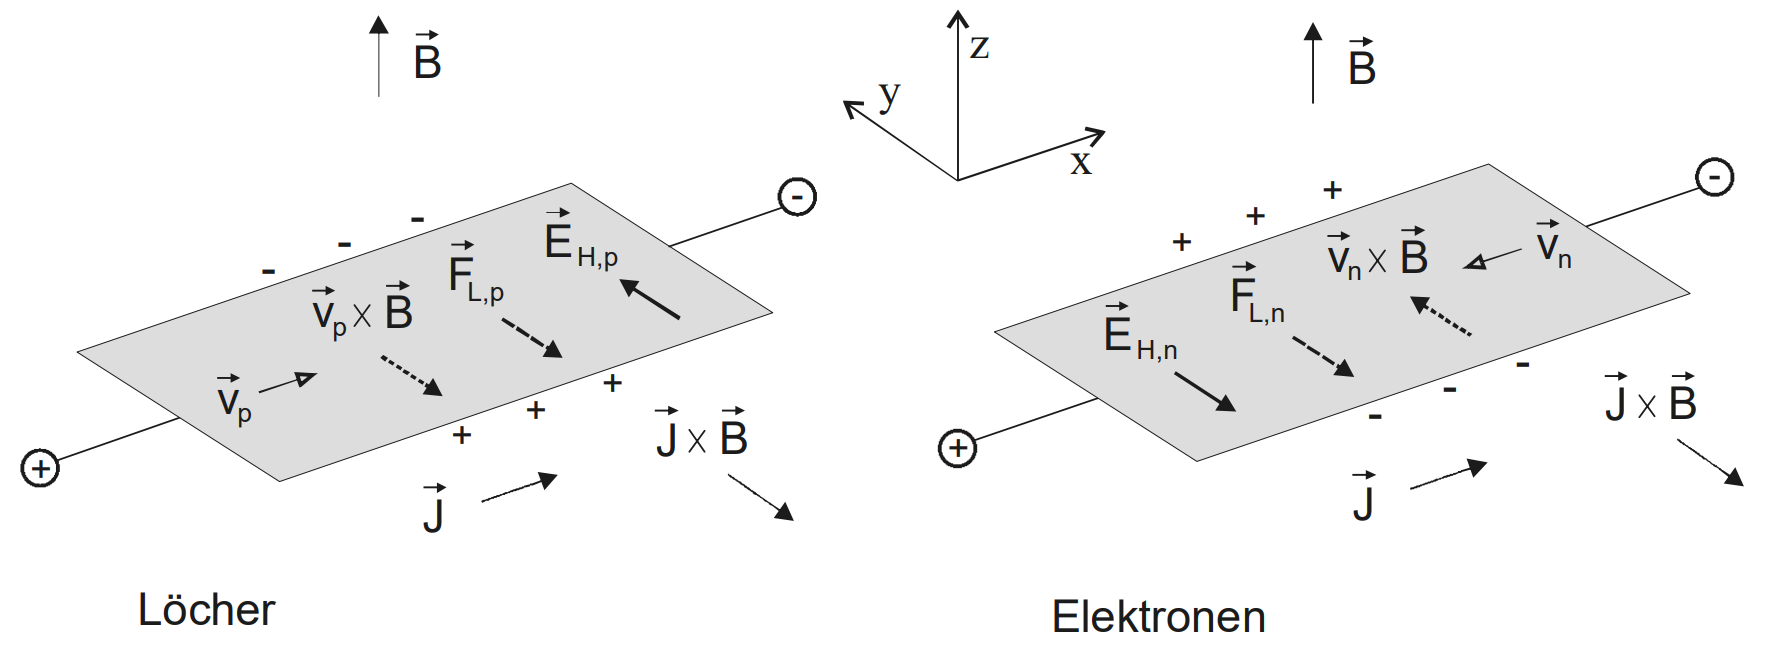
\includegraphics[width=1.0\textwidth]{./fig/bipo_hall.png}
    \label{fig:bihl}
\end{figure}
Betrachtet man nun auch Löcher als Ladungsträger wie im Halbleiter nennt man die Leitung bipolar. Löcher haben dabei positive Ladung, aber auch die entgegengesetzte Geschwindigkeit zu Elektronen, daher wirkt die Lorenzkraft in die selbe Richtung. Auch die Stromdichte verläuft in die selbe Richtung wie bei Elektronen. Das Hall-Feld ist jedoch antiparallel aber der Vektor $( \Vec{J} \times \Vec{B} )$ ist parallel, darausf folgt:
\begin{align}
    ( \Vec{J} \times \Vec{B} ) = (-J_x B_z) ê_y \\
    \Vec{E}_H = \pm |E_H| ê_y.
\end{align}
Die Hall-Konstante ist damit:
\begin{align}
    R_H = \frac{\pm|E_H|}{J_xB_z}
\end{align}
und die Stromdichte im bipolaren Fall:
\begin{align}
    J_x = |e| \cdot (n\mu_n+p\mu_p) \cdot E_x
\end{align}
Schlussendlich folgt für die bipolare Hall-Konstante:
\begin{align}
    R_H^{bipolar} = \frac{p-nb^2}{|e|(p+nb)^2} \\
    b= \frac{\mu_n}{\mu_p}
\end{align}
Das Produkt $\sigma |R_H|$ enstpricht dabei im unipolaren Fall der Beweglichkeit und im bipolaren Fall der Differenz der Beweglichkeiten:
\begin{align}
    \mu_n &= \sigma |R_H| \qquad (extrinsisch) \\
    \mu_n - \mu_p &= \sigma |R_H| \qquad (intrinsisch)
\end{align}
